\documentclass[a4paper,10pt]{beamer}

\usepackage{media9}

\usepackage{hyperref}
\usepackage[export]{adjustbox}

\usetheme{Darmstadt}
\useinnertheme{default}
\useoutertheme[footline=empty,subsection=false]{miniframes}
\setbeamertemplate{frametitle}[default][center]
\setbeamertemplate{itemize items}[square]

\setbeamertemplate{blocks}[default]

%\setbeamertemplate{footline}[frame number]
\setbeamertemplate{footline}[text line]{%
}

\setbeamertemplate{background}{%
	\put(5,-270){%
		\parbox{1.16\linewidth}{\tiny Presentation Project: Chat System - GUI, Game, File System \& Process \hfill \raggedleft\insertframenumber~/ \inserttotalframenumber}
	}
	
}

\setbeamercovered{transparent}

\setbeamertemplate{navigation symbols}{}

\setbeamercolor{block title alerted}{use=structure,fg=white,bg=orange!75!black}
\setbeamercolor{block body alerted}{use=structure,fg=black,bg=orange!10!white}

\setbeamercovered{invisible}

\setbeamertemplate{frametitle}
{
	\nointerlineskip
	\begin{beamercolorbox}[sep=0.3cm,ht=1.8em,wd=\paperwidth]{frametitle}
		\vbox{}\vskip-2ex%
		\strut\vspace*{-0.85cm}\insertframetitle\strut
		\hfill
		\raisebox{-1cm}{
\includegraphics[scale=0.05,trim={0cm 0cm 0 0cm},clip]{logo2_NYU.jpg}}
		\vskip-0.8ex%
	\end{beamercolorbox}
}

\usepackage{graphicx}
\usepackage{amsmath,amssymb}
\usepackage[latin1]{inputenc}
\usepackage{psfrag}
\usepackage{pgf}
\usepackage{minted}
\usepackage{xcolor}
\usepackage{tcolorbox}
\usepackage{textcomp}
\usepackage{upquote}
\usepackage{media9}


\AtBeginDocument{%
	\def\PYZsq{\textquotesingle}%
}

\usemintedstyle{default}

\usepackage{tikz}
\usetikzlibrary{shapes.geometric, arrows, positioning, shapes.multipart}

\tikzstyle{startstop} = [rectangle, rounded corners, minimum width=2cm, minimum height=1cm,text width=2cm,text centered, draw=black, fill=red!30]
\tikzstyle{process} = [rectangle, minimum width=2cm, minimum height=1cm, text centered, text width=2cm, draw=black, fill=orange!30]
\tikzstyle{decision} = [diamond,aspect=3, minimum width=2cm, minimum height=1cm, text width=2cm,inner sep=0pt,text centered, draw=black, fill=green!30]
\tikzstyle{decision_text} = [rectangle, minimum width=2cm, minimum height=1cm, text width=2cm,inner sep=0pt,text centered]
\tikzstyle{box} = [rectangle, minimum width=0.5cm, minimum height=0.5cm, text width=0.5cm,inner sep=0pt,text centered,draw=black, fill=gray!30]
\tikzstyle{io} = [trapezium, trapezium left angle=70, trapezium right angle=110, trapezium stretches=true,minimum width=2cm, minimum height=1cm, text centered, text width=2cm, draw=black, fill=blue!30]
\tikzstyle{func} = [rectangle split, rectangle split horizontal,rectangle split parts=3,minimum height=1cm, text centered, draw=black, fill=yellow!30,rectangle split empty part width=-6pt]


\tikzstyle{arrow} = [thick,->,>=stealth]

\newcommand\myrule[1]{\multicolumn{1}{c|}{#1}}

\definecolor{light-blue}{RGB}{173,216,230}
\definecolor{yellow}{RGB}{255,255,0}
\definecolor{light-gray}{gray}{0.8}

\newtcbox{\mybox}{nobeforeafter,colback=light-gray,boxrule=0pt,arc=4pt,
	boxsep=0pt,left=6pt,right=6pt,top=6pt,bottom=6pt,width=\width}
\tcbset{ boxrule=0pt,fontupper=\normalsize,colback=light-gray,width=\linewidth,after={\par\noindent}}


\tikzstyle{mybox} = [draw=black, fill=yellow, thick,
rectangle,  inner sep=10pt, inner ysep=20pt]
\tikzstyle{fancytitle} =[fill=black, text=white]


\title{Presentation Project: Chat System\\-\\GUI, Game, File System \& Process}

\author{James Chen \& Shanglin Yang}


\institute{
\includegraphics[scale=0.4]{logo_NYU.png}}

\date{Instructors: Prof. Xianbin Gu \& Dr. Wen Yin}

%\logo{
\includegraphics[scale=0.04]{logo2_NYU.jpg}}


\begin{document}


%%%%%%%%%%%%%%%%%%%%%%%%%%%%%%%%%%%%%%%%%%%%%%%%%%%%%%%%%%%%%%%%%%%%%%%%%%%%%%%%%%%%%%%%%%%%%%%%%%%%%%%%%%%%%
%%%%%%%%%%%%%%%%%%%%%%%%%%%%%%%%%%%%%%%%%%%%%%%%%%%%%%%%%%%%%%%%%%%%%%%%%%%%%%%%%%%%%%%%%%%%%%%%%%%%%%%%%%%%%
\frame[plain]{
	\titlepage
}

\section{Introduction}

\begin{frame}{Introduction}
\begin{block}{Have You Ever Experience Situations Like This ... }
\begin{center}
\begin{minipage}[t]{0.6\textwidth}
\centering
\begin{figure}[H]
    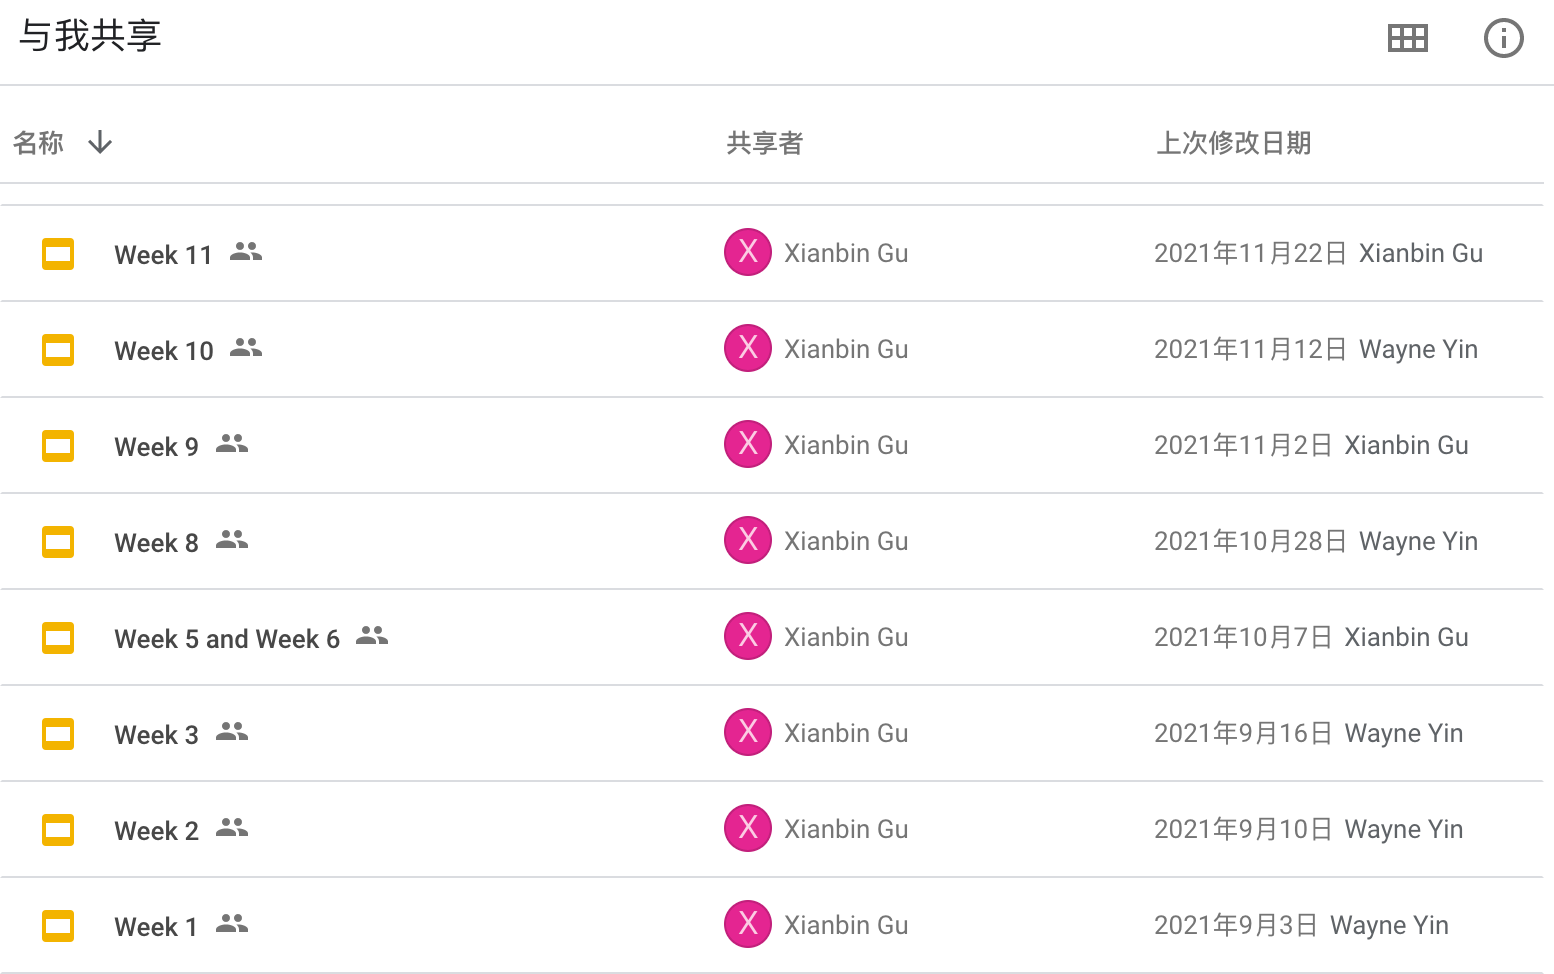
\includegraphics[width=\textwidth]{intro.png}
\end{figure}
\end{minipage}
\begin{minipage}[t]{0.35\textwidth}
\centering
\begin{figure}[H]
    \centering
    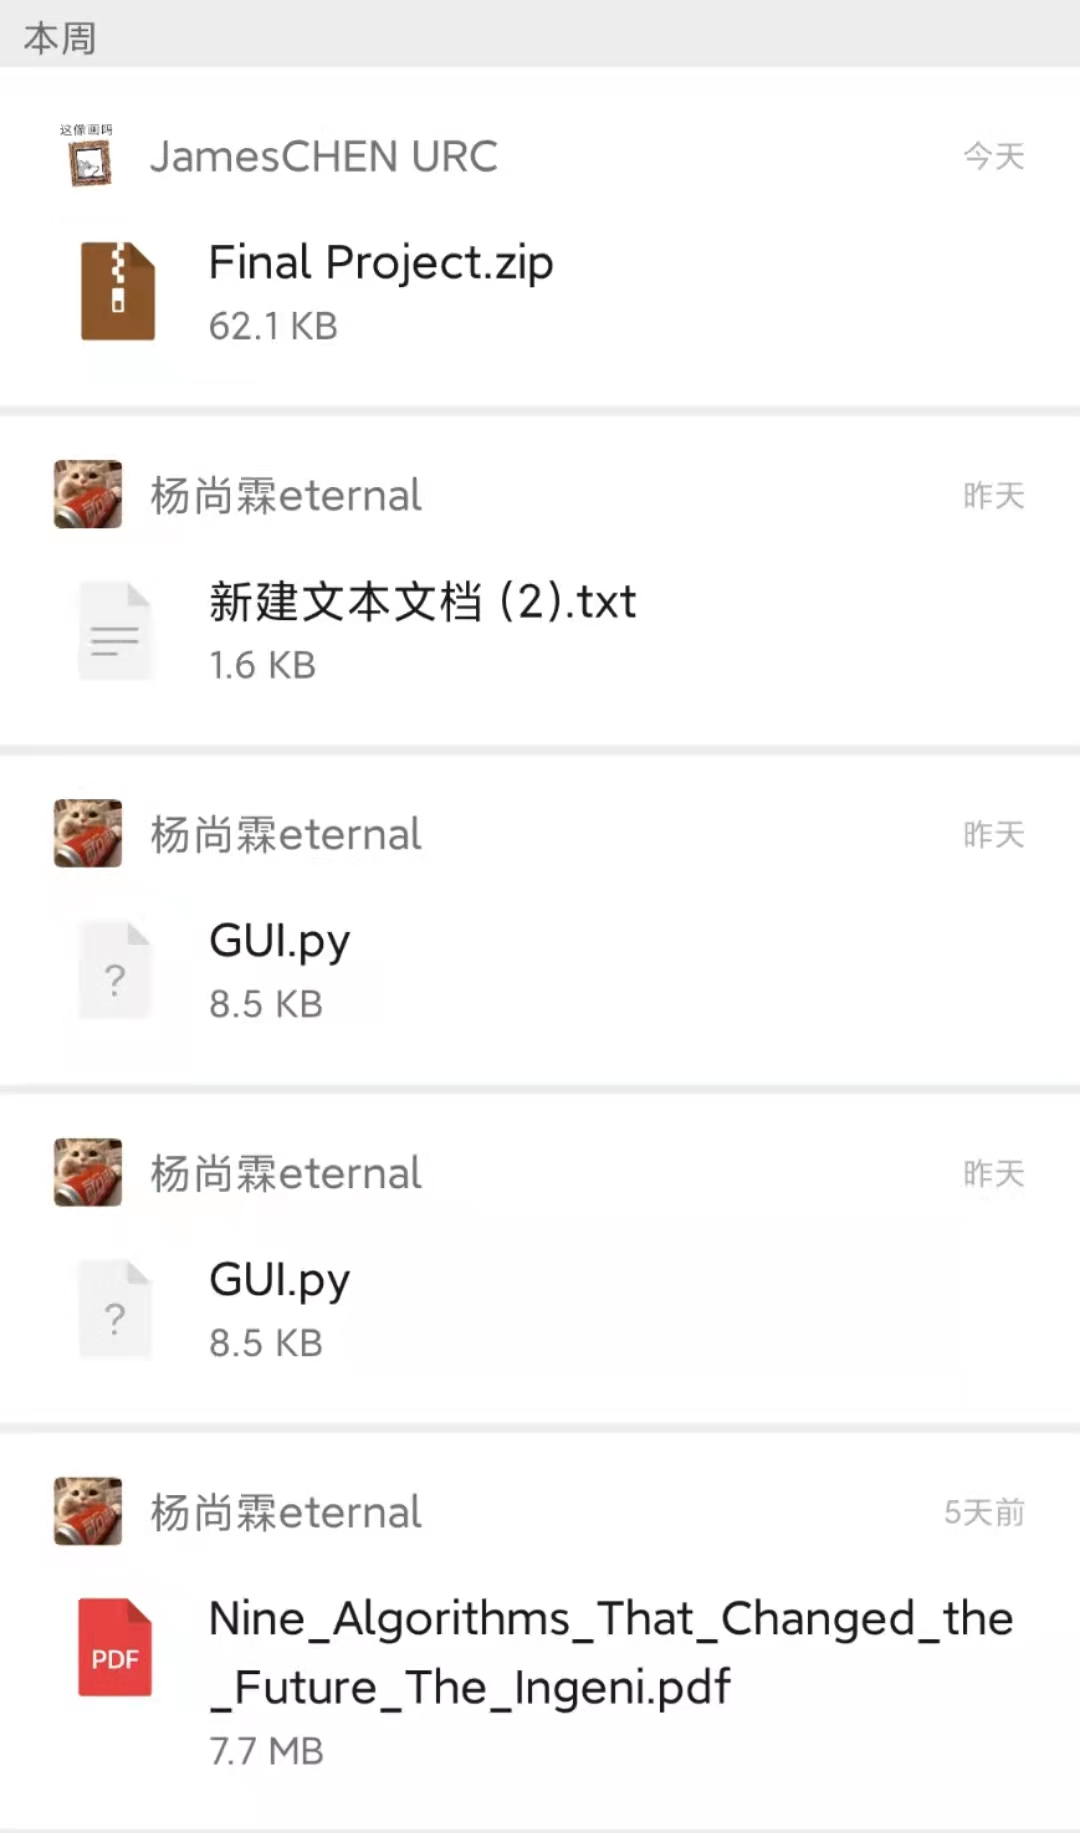
\includegraphics[width=0.8\textwidth]{intro.jpeg}
\end{figure}
\end{minipage}
\end{center}
\end{block}
\end{frame}

\begin{frame}{Introduction}
\begin{block}{Have You Ever Experience Situations Like This ... }
\begin{figure}[H]
    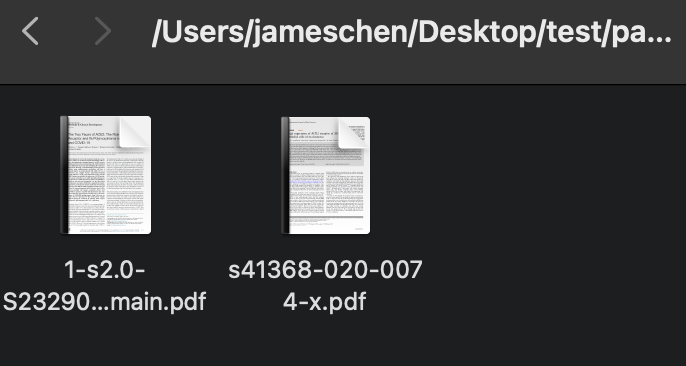
\includegraphics[width=\textwidth]{file_rename.png}
\end{figure}
\end{block}
\end{frame}

\begin{frame}{Introduction}
\begin{block}{Have You Ever Experience Situations Like This ... }
\begin{figure}[H]
    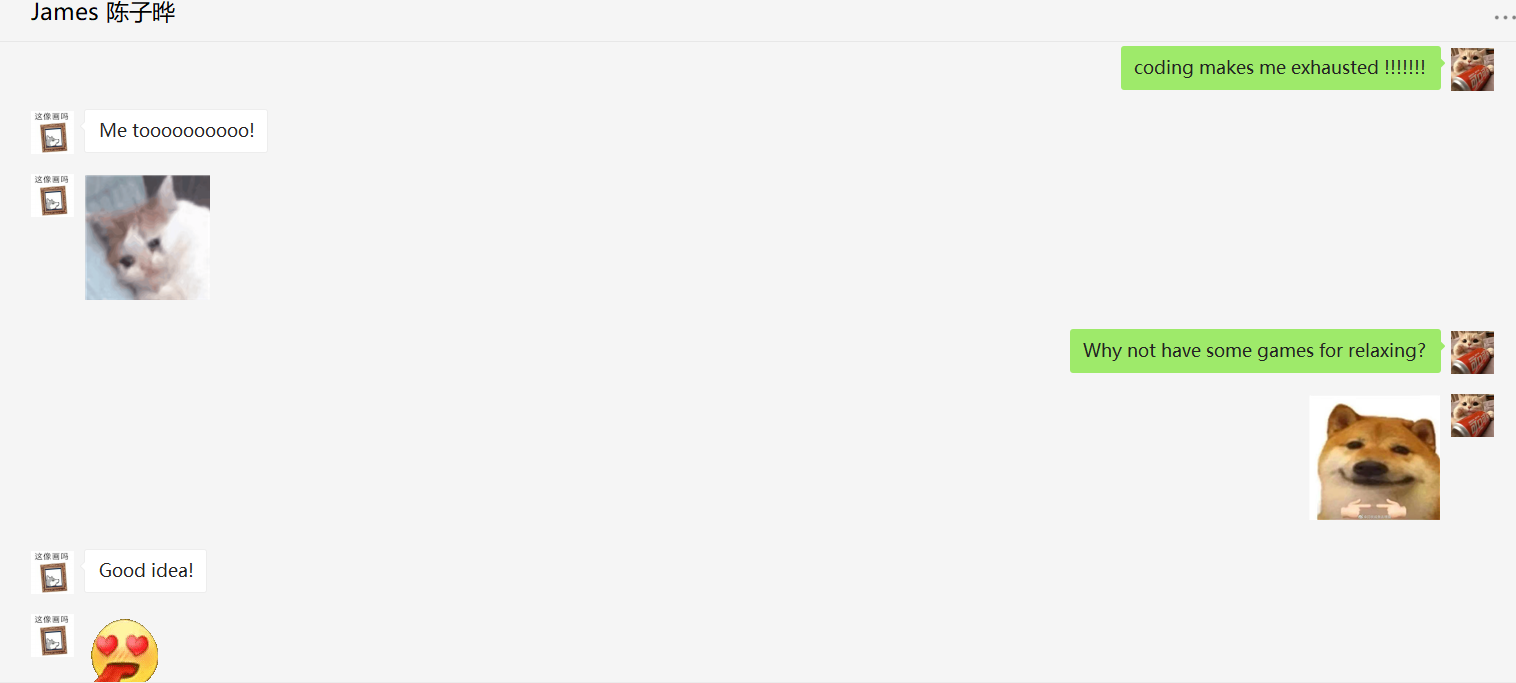
\includegraphics[width=\textwidth]{game123.png}
\end{figure}
\end{block}
\end{frame}

\begin{frame}{Introduction}
\begin{block}{Our Modification to the Chat System}
\begin{itemize}
		\item Graphical User Interface
		\item Game
		\item FTP Server: File Upload \& Download
		\item PDF Rename
\end{itemize}
\end{block}
\end{frame}


\section{Graphical User Interface}
\begin{frame}{Sections}
\begin{block}{Our Modification to the Chat System}
\begin{itemize}
		\item \textbf{Graphical User Interface}
		\item Game
		\item FTP Server: File Upload \& Download
		\item PDF Rename
\end{itemize}
\end{block}
\end{frame}

\begin{frame}{Graphical User Interface}
\begin{block}{Additional Buttons and Location Adjustment}
\begin{figure}
    \centering
    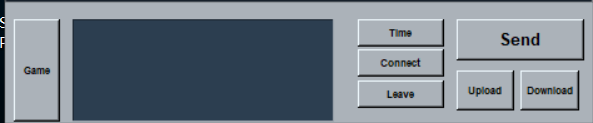
\includegraphics[width=0.85\linewidth]{surface.png}
\end{figure}
\end{block}
\end{frame}

\begin{frame}{Graphical User Interface}

\begin{block}{Time Button}
\begin{figure}
    \centering
    
\includegraphics[width=0.3\linewidth]{time.png}
\end{figure}
	\inputminted[linenos]{python}{time.py}
\end{block}
\end{frame}

\begin{frame}{Graphical User Interface}
\begin{block}{Connect Button}
\begin{figure}
    \centering
    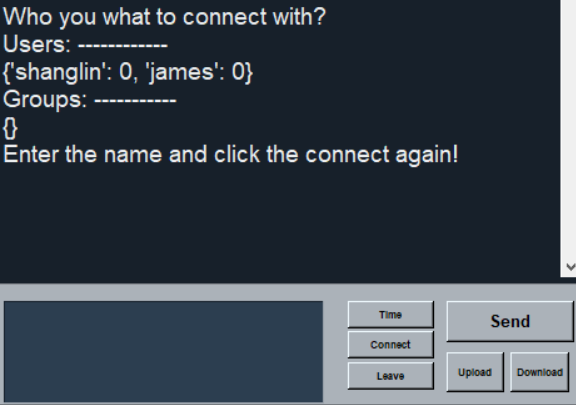
\includegraphics[width=0.7\linewidth]{connect1.png}
\end{figure}
\end{block}
\end{frame}

\begin{frame}{Graphical User Interface}
\begin{block}{Connect Button}
\begin{figure}
    \centering
    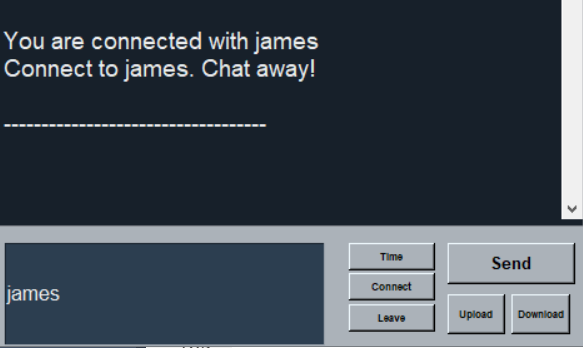
\includegraphics[width=0.7\linewidth]{connect2.png}
\end{figure}
\end{block}
\end{frame}

\begin{frame}{Graphical User Interface}
\begin{block}{Connect Button}
\inputminted[linenos]{python}{connect.py}
\end{block}
\end{frame}


\begin{frame}{Graphical User Interface}
\begin{block}{Leave Button}
\inputminted[linenos]{python}{quit.py}
\end{block}
\end{frame}

\begin{frame}{Graphical User Interface}
\begin{block}{Upload Button}
\begin{figure}
    \centering
    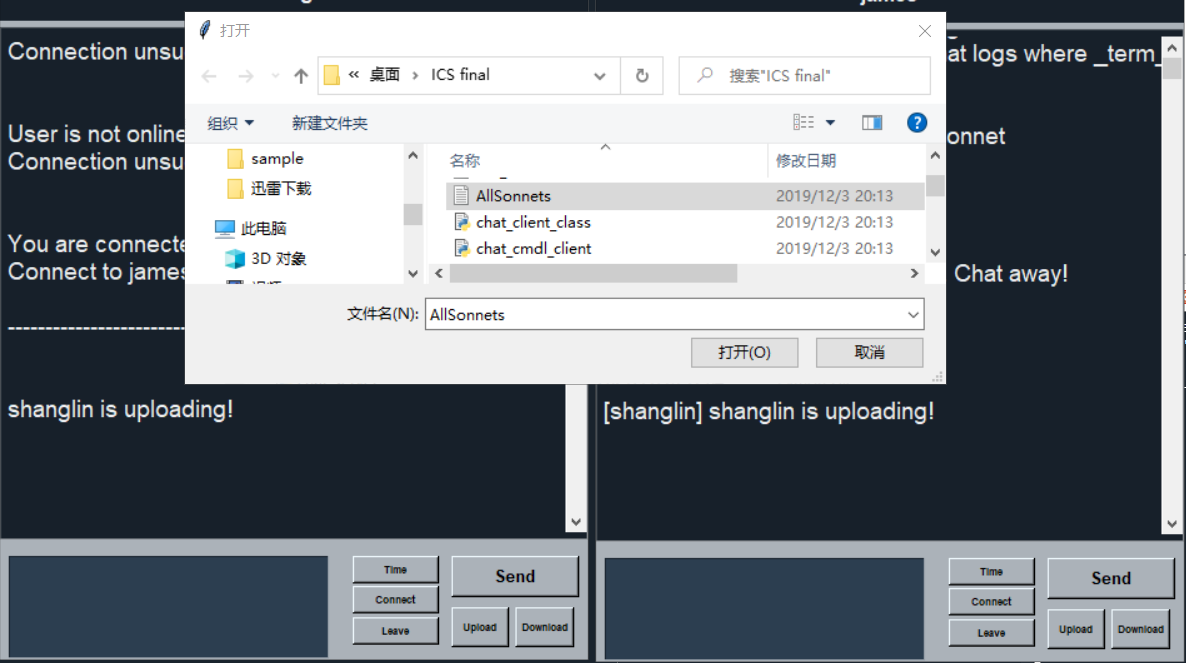
\includegraphics[width=\linewidth]{upload.png}
\end{figure}
\end{block}
\end{frame}

\begin{frame}{Graphical User Interface}
\begin{block}{Upload Button}
\inputminted[linenos]{python}{upload.py}
\end{block}

\end{frame}

\section{Game}
\begin{frame}{Sections}
\begin{block}{Our Modification to the Chat System}
\begin{itemize}
		\item Graphical User Interface
		\item \textbf{Game}
		\item FTP Server: File Upload \& Download
		\item PDF Rename
\end{itemize}
\end{block}
\end{frame}

\begin{frame}{Game}
\begin{block}{Game demo}
\begin{figure}[H]
    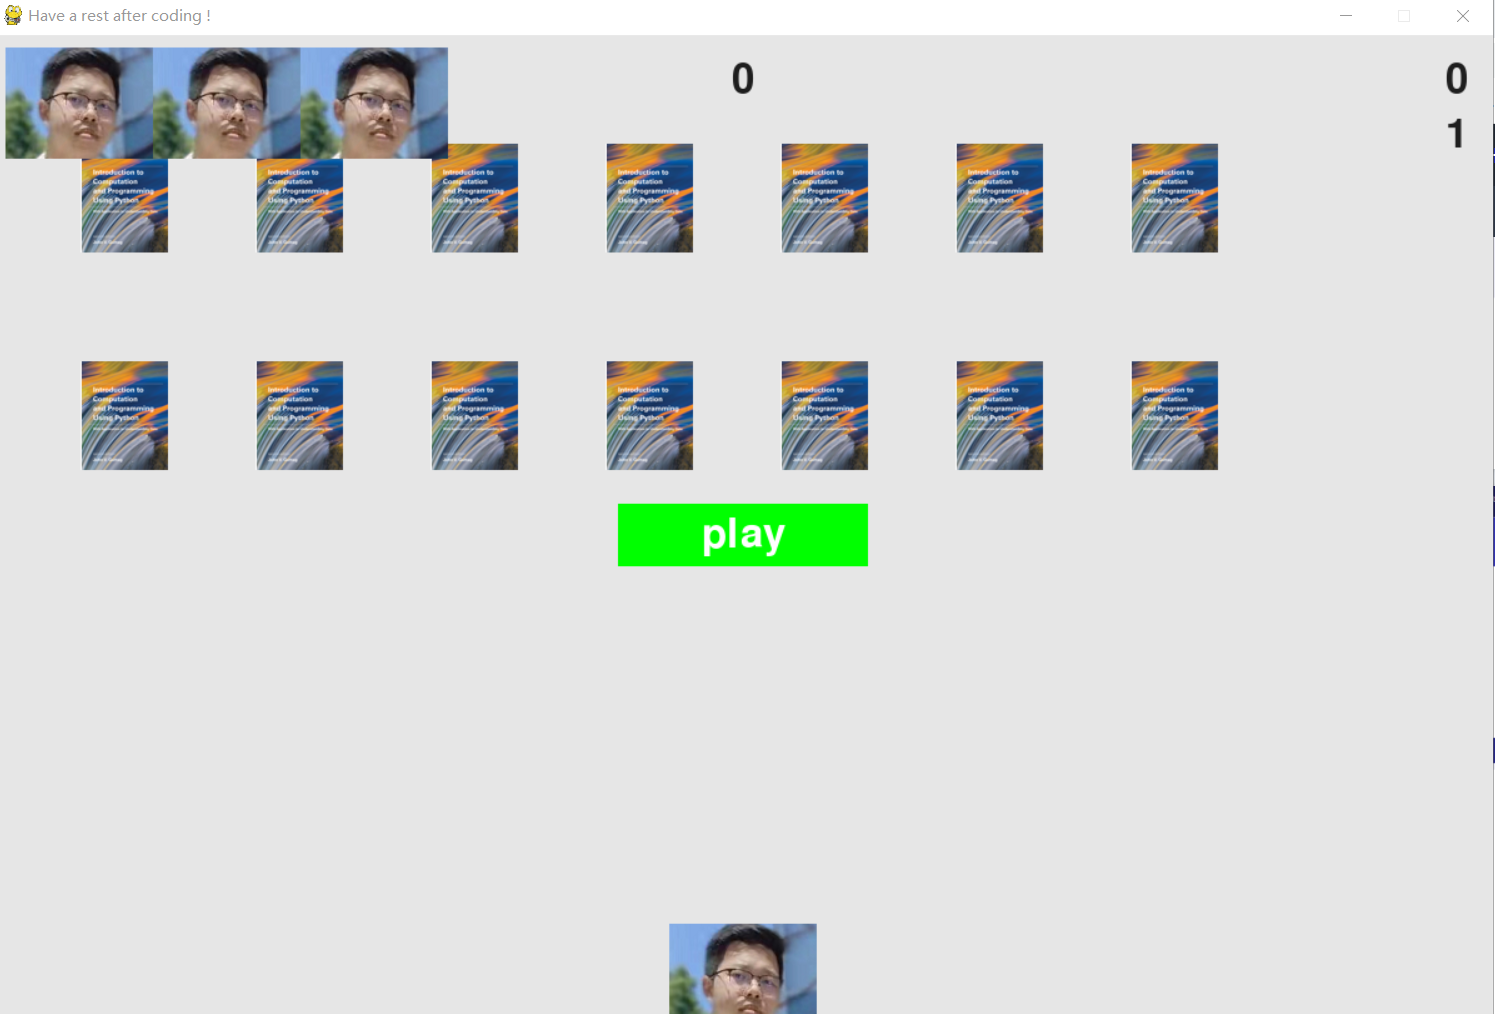
\includegraphics[width=0.8\textwidth]{game3.png}
\end{figure}
\end{block}
\end{frame}

\begin{frame}{Game}
\begin{minipage}[t]{0.45\textwidth}
\flushleft{
\begin{figure}[H]
    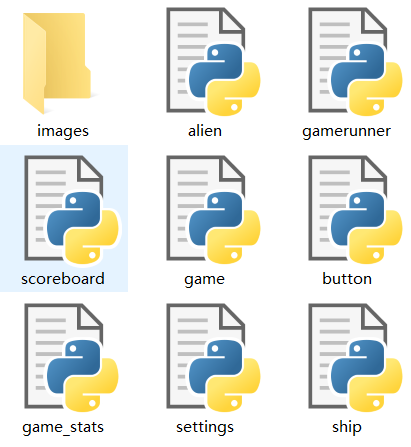
\includegraphics[width=0.8\textwidth]{game2.png}
\end{figure}}
\end{minipage}
\begin{minipage}[t]{0.5\textwidth}
\begin{block}{Code overview}
\begin{center}
\centering
\inputminted[linenos]{python}{pakage.py}
\end{center}
\end{block}
\end{minipage}
\end{frame}

\begin{frame}{Game}
\begin{block}{Intialization}
\inputminted[linenos]{python}{init1.py}
\end{block}
\end{frame}

\begin{frame}{Game}
\begin{block}{Updating the screen}
\inputminted[linenos]{python}{update1.py}
\end{block}
\end{frame}

\begin{frame}{Game}
\begin{block}{Setting file}
\inputminted[linenos]{python}{settings1.py}
\end{block}
\end{frame}

\section{FTP Server: File Upload \& Download}

\begin{frame}{Sections}
\begin{block}{Our Modification to the Chat System}
\begin{itemize}
		\item Graphical User Interface
		\item Game
		\item \textbf{FTP Server: File Upload \& Download}
		\item PDF Rename
		
\end{itemize}
\end{block}
\end{frame}

\begin{frame}{FTP Server: File Upload \& Download}
\begin{block}{Structure}
\begin{figure}[H]
    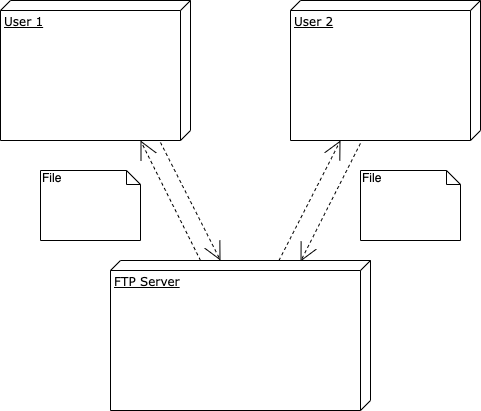
\includegraphics[width=0.6\textwidth]{Structure.png}
\end{figure}
\end{block}
\end{frame}

\begin{frame}{FTP Server: File Upload \& Download}
	\begin{block}{FTP Server}
	\inputminted[linenos]{python}{file_server.py}
	\end{block}
\end{frame}

\begin{frame}{FTP Server: File Upload \& Download}
	\begin{block}{Threading (in chat\_server)}
	\inputminted[linenos]{python}{threading.py}
	\end{block}
\end{frame}

\begin{frame}{FTP Server: File Upload \& Download}
	\begin{block}{Upload (in GUI)}
	\inputminted[linenos]{python}{file_upload.py}
	\end{block}
\end{frame}

\begin{frame}{FTP Server: File Upload \& Download}
\begin{block}{Download (in GUI)}
	\inputminted[linenos]{python}{download.py}
\end{block}  
\end{frame}

\section{PDF Rename}
\begin{frame}{Sections}
\begin{block}{Our Modification to the Chat System}
\begin{itemize}
		\item Graphical User Interface
		\item Game
		\item FTP Server: File Upload \& Download
		\item \textbf{PDF Rename}
\end{itemize}
\end{block}
\end{frame}

\begin{frame}{PDF Rename}
\begin{block}{PDF Rename: Library \& Path}
	\inputminted[linenos]{python}{PDF1.py}
\end{block}
\end{frame}

\begin{frame}{PDF Rename}
\begin{block}{PDF Rename: File Process}
	\inputminted[linenos]{python}{PDF2.py}
\end{block}
\end{frame}

\begin{frame}{PDF Rename}
\begin{block}{PDF Rename: Demo -- Before}
\begin{figure}[H]
    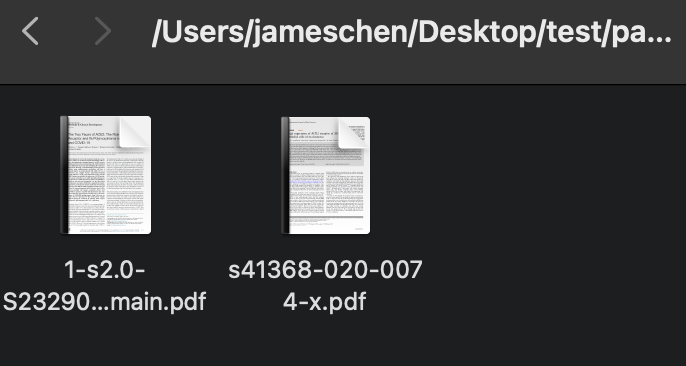
\includegraphics[width=\textwidth]{file_rename.png}
\end{figure}
\end{block}
\end{frame}

\begin{frame}{PDF Rename}
\begin{block}{PDF Rename: Demo -- After}
\begin{figure}[H]
    
\includegraphics[width=\textwidth]{file_rename_after.png}
\end{figure}
\end{block}
\end{frame}

\section{Possible Improvements}
\begin{frame}{Possible Improvements}
\begin{block}{Possible Improvements}
\begin{itemize}
		\item Authority Management
		\item Secure Messaging
\end{itemize}
\end{block}
\end{frame}


\section{Acknowledgments}
\begin{frame}{Acknowledgments}
\begin{block}{Acknowledgments}
We would like to express our sincere gratitude to our main instructor Prof. Xianbin Gu, teaching assistant Dr. Wen Yin. Without their instruction, this project would not have been accomplished. Special thanks to GitHub user @wolfpan for insightful suggestions for debugging. Thanks Prof. Lihua Xu for providing this very handy \LaTeX template.
\end{block}
\end{frame}

\section{References}
\begin{frame}{References}
\begin{block}{Bibliography}
\begin{enumerate}
\item 61MKSI, "Python builds an ftp server in one second to help you share files on the LAN" \textit{Zhihu}. [Online]. Available: https://zhuanlan.zhihu.com/p/84228436. 
\item ChangTingWai, "Python- upload a single file to FTP" \textit{Zhihu}. [Online]. Available: https://zhuanlan.zhihu.com/p/415360923.
\item royal, "Use python to read pdf titles and categorize them" \textit{CSDN}. [Online]. Available: https://blog.csdn.net/weixin\_41090039/article/details/82421312.
\item Shawpan, "Python one sentence using the file dialog to get the file path" \textit{CSDN}. [Online]. Available: https://blog.csdn.net/shawpan/article/details/78759199. 
\item T. Gaddis, \textit{Starting out with python}. Harlow, United Kingdom: Pearson, 2022. 
\end{enumerate}
\end{block}
\end{frame}

\end{document}